%===============================================================
% Template author: Martin Malý.
% Template URL: https://www.overleaf.com/latex/templates/czech-technical-university-colors-beamer-template-lab-of-structure-of-biomolecules/xmgmzfhtyrxt
%===============================================================

\documentclass{beamer}
% \documentclass[aspectratio=169]{beamer} % Uncomment for 16:9
\usepackage[utf8]{inputenc}

\usetheme{Madrid}

\definecolor{cvut_navy}{HTML}{0065BD}
\definecolor{cvut_blue}{HTML}{6AADE4}
\definecolor{cvut_gray}{HTML}{156570}

\setbeamercolor{section in toc}{fg=black,bg=white}
\setbeamercolor{alerted text}{fg=cvut_blue}
\setbeamercolor*{palette primary}{bg=cvut_navy,fg=gray!20!white}
\setbeamercolor*{palette secondary}{bg=cvut_blue,fg=white}
\setbeamercolor*{palette tertiary}{parent=palette primary}
\setbeamercolor*{palette quaternary}{fg=green,bg=gray!5!white}

\setbeamercolor*{sidebar}{fg=cvut_navy,bg=gray!15!white}


\setbeamercolor{titlelike}{parent=palette primary}
\setbeamercolor{frametitle}{parent=palette primary}

\setbeamercolor*{separation line}{}
\setbeamercolor*{fine separation line}{}

\setbeamertemplate{navigation symbols}{}

% Change itemize and enumerate style.
\setbeamertemplate{itemize item}{%
  \textcolor{cvut_navy}{\raisebox{.45ex}{\rule{.8ex}{.8ex}}}
}
\setbeamertemplate{enumerate item}{%
  \textcolor{cvut_navy}{\arabic{enumi}.}
}

\usepackage{eqnarray,amsmath}
\usepackage{amsfonts}
\usepackage{amssymb}
\usepackage{graphicx}
\usepackage{lmodern} % for bold and italic at the same time
\usepackage{bm} % for bold and italic at the same time
\usepackage{epstopdf}
\usepackage{changepage}
\usepackage{array,booktabs}
\usepackage[dua, nolist]{acronym}

%% | -------------------------- tikz -------------------------- |

\usepackage{tikz}
\usepackage{pgfplots}
\pgfplotsset{compat=1.14}
\usetikzlibrary{backgrounds,arrows,automata,shapes,positioning,calc,through,spy,shapes,shapes.geometric,shapes.multipart,fit,patterns,fadings}
\pgfdeclarelayer{background}
\pgfdeclarelayer{foreground}
\pgfsetlayers{background,main,foreground}
\tikzset{
    use page relative coordinates/.style={
        shift={(current page.south west)},
        x={(current page.south east)},
        y={(current page.north west)}
    },
}


% Change color of Figure and Table labels.
\usepackage[labelfont={color=cvut_navy}]{caption}

% Define logo condition
\newif\ifplacelogo
\logo{\ifplacelogo
\includegraphics[height=1cm]{src/fig/pdfs/ctu_logo_blue_filled.pdf}\fi}


%====================================================
%========== DEFINITION OF AUTHORS ETC...=============
%====================================================
\author[Yauheni Zviazdou]{Yauheni Zviazdou}
\institute[]{Czech Technical University in Prague \\ Faculty of Electrical Engineering \\ Department of Cybernetics \\}
\title[Text representation models. RAG.]{From FastText to Transformer Models, and their Application in Retrieval-Augmented Generation}
\date[Bachelor's thesis presentation]{Bachelor's thesis presentation\\Supervisor: Ing. Jan Šedivý, CSc.}

%====================================================
%========== BEGINNING OF DOCUMENT ===================
%====================================================
\begin{document}


% Title slide
\begin{frame}
  \titlepage
  \begin{center}
    
\includegraphics[height=2cm]{src/fig/pdfs/ctu_logo_blue_filled.pdf}
  \end{center}
  %!TEX root = ../main.tex

\begin{acronym}
  \acro{CTU}[CTU]{Czech Technical University}
  \acro{API}[API]{Application Programming Interface}
  \acro{RAG}[RAG]{Retrieval-Augmented Generation}
  \acro{NLP}[NLP]{Natural Language Procession}
  \acro{STS}[STS]{Semantic Textual Similarity}
  \acro{QA}[QA]{Question Answering}
  \acro{BERT}[BERT]{Bidirectional Encoder Representations from Transformers}
  \acro{CBOW}[CBOW]{Continuous Bag-of-Words}
  \acro{GloVe}[GloVe]{Global vectors}
  \acro{ML}[ML]{Machine Learning}
  \acro{NN}[NN]{Neural Network}
  \acro{BoW}[BoW]{Bag-of-Words}
  \acro{TF-IDF}[TF-IDF]{Term Frequency-Inverse Document Frequency}
  \acro{OOV}[OOV]{Out of vocabulary}
\end{acronym}

\end{frame}


% Motivation
\placelogotrue
\begin{frame}
  \frametitle{Motivation}
  \begin{columns}
    \begin{column}{0.5\textwidth}
      \begin{itemize}
        \item LLM chatbots integrate external documents, enhancing context-aware responses.
        \item Answer quality depends on the context provided by the technical document.
        \item Context quality depends on text representation.
      \end{itemize}
    \end{column}
    \begin{column}{0.5\textwidth}
      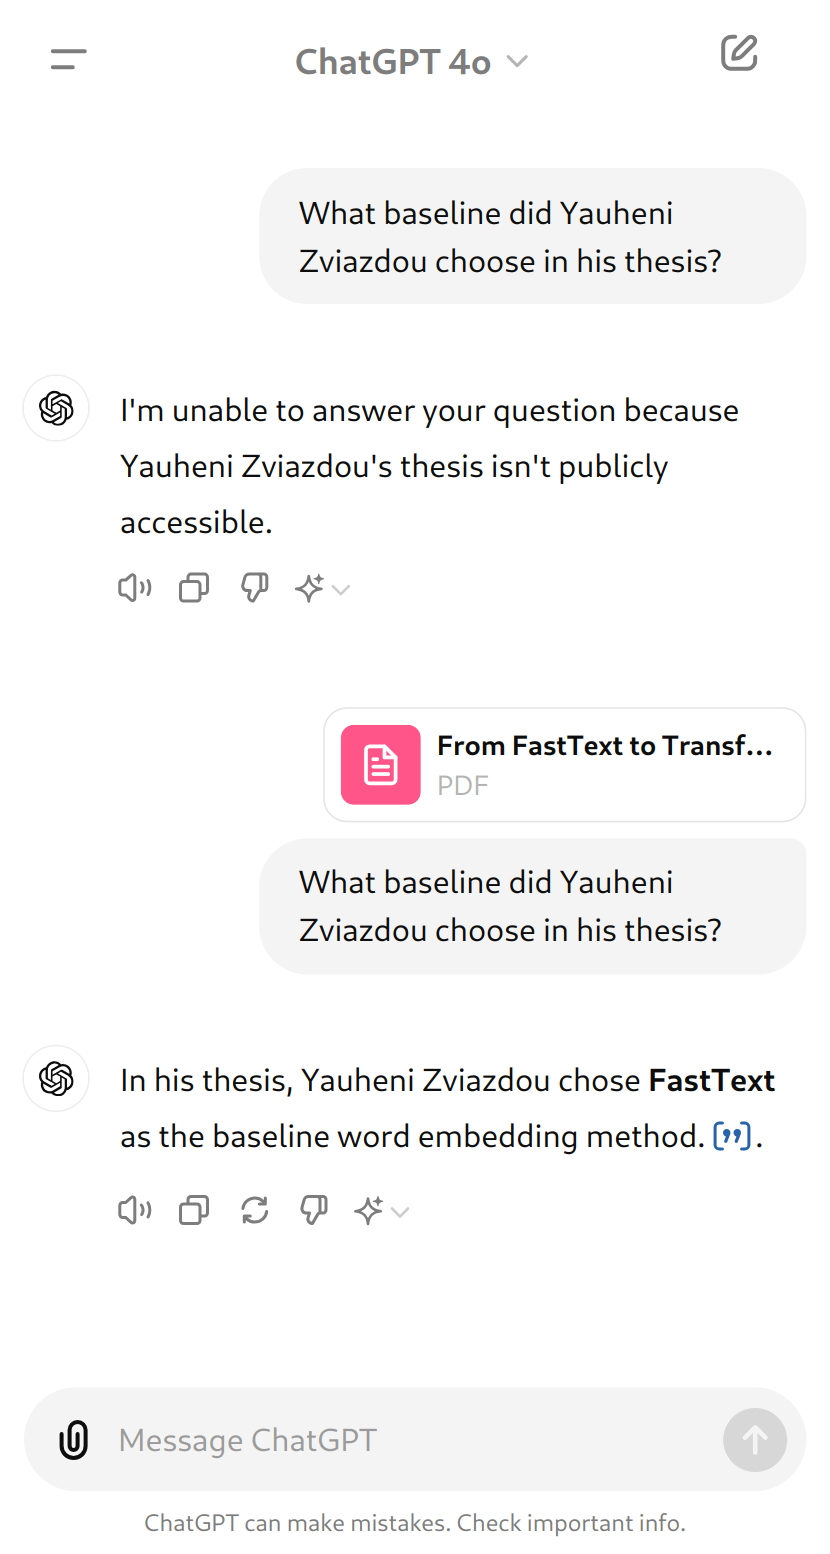
\includegraphics[scale=0.15]{src/fig/imgs/RAG_example.png}
    \end{column}
  \end{columns}

  % Adding cross and check marks.
  % https://tex.stackexchange.com/questions/42619/xmark-that-complements-the-ams-checkmark
  \newcommand{\tikzxmark}{%
  \tikz[scale=0.02] {
      \draw[line width=1.2,line cap=round] (0,0) to [bend left=6] (1,1);
      \draw[line width=1.2,line cap=round] (0.2,0.95) to [bend right=3] (0.8,0.05);
  }}
  \newcommand{\tikzcmark}{%
  \tikz[scale=0.02] {
      \draw[line width=1.2,line cap=round] (0.25,0) to [bend left=10] (1,1);
      \draw[line width=1.3,line cap=round] (0,0.35) to [bend right=1] (0.23,0);
  }}
  \begin{tikzpicture}[remember picture, overlay,use page relative coordinates]
    \node at (0.90,0.63) {\tikzxmark};
    \node at (0.90,0.27) {\tikzcmark};
      
  \end{tikzpicture}
\end{frame}


% Work objectives
\begin{frame}
  \frametitle{Work objectives}
  \textcolor{cvut_navy}{\textbf{Task 1.}} Review and compare text representation methods.
  \begin{itemize}
    \item Review text representation methods.
    \item Compare traditional and transformer-based methods.
  \end{itemize}
  \textcolor{cvut_navy}{\textbf{Task 2.}} RAG Optimization
  \begin{itemize}
    \item Choose optimal models for RAG.
    \item Choose optimal chunk size and number of context chunks.
  \end{itemize}
  \bigskip
  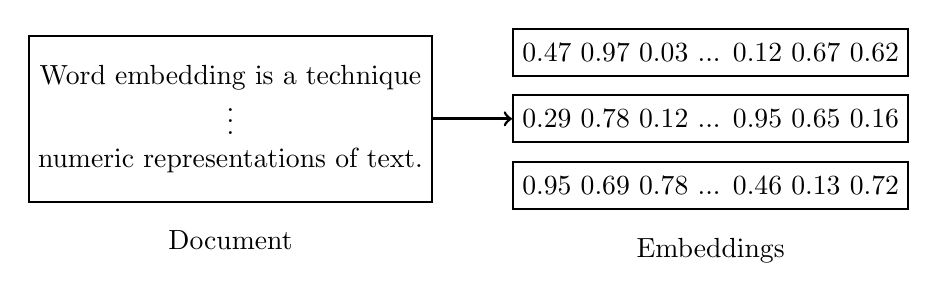
\begin{tikzpicture}[
    longnode/.style={rectangle, draw=black, thick, align=left, minimum height=1.7em, minimum width=14em},
    highnode/.style={longnode, minimum height=6em},
    line width=1pt, black
    ]
    
    %Nodes
    \node[highnode, align=center] (text) []                              {Word embedding is a technique\\ \vdots \\numeric representations of text.};
    \node[longnode, align=center] (emb2) [right=of text]                 {0.29 0.78 0.12 ... 0.95 0.65 0.16};
    \node[longnode, align=center] (emb3) [below=of emb2,yshift=+2.221em] {0.95 0.69 0.78 ... 0.46 0.13 0.72};
    \node[longnode, align=center] (emb1) [above=of emb2,yshift=-2.221em] {0.47 0.97 0.03 ... 0.12 0.67 0.62};

    % Text labels (outside nodes)
    \node[below=of text, yshift=+2.221em]     {Document};
    \node[below=of emb3, yshift=+2.221em]     {Embeddings};

    %Lines
    \draw[->] (text.east) -- (emb2.west);
\end{tikzpicture}

\end{frame}


% Text representation methods
\begin{frame}[t]
  \frametitle{Text representation methods}
  \begin{columns}[onlytextwidth]
    \begin{column}{0.5\textwidth}
      \begin{figure}
        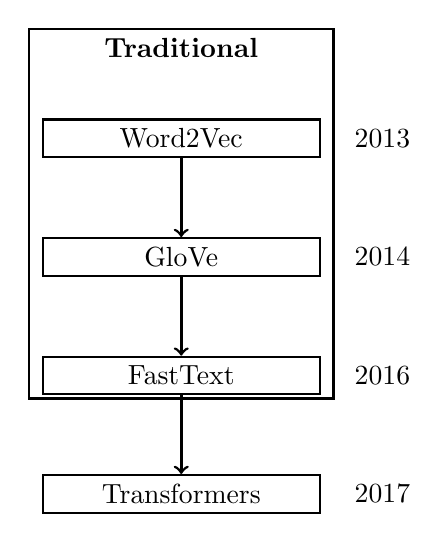
\begin{tikzpicture}[line width=1pt, black]
    %Nodes
    \begin{scope}[every node/.style={rectangle, draw=black, thick, align=left, minimum width=10em}]
    \node (Word2Vec)     []                  {Word2Vec};
    \node (GloVe)        [below=of Word2Vec] {GloVe};
    \node (FastText)     [below=of GloVe]    {FastText};
    \node (Transformers) [below=of FastText] {Transformers};
    \end{scope}

    \node (traditional) [rectangle, draw=black, text depth = 12em, anchor=north, minimum width=11em, yshift=+4em]{\textbf{Traditional}};


    % Text labels (outside nodes)
    \node[right=of Word2Vec.east,xshift=-2.em]     {2013};
    \node[right=of GloVe.east,xshift=-2.em]        {2014};
    \node[right=of FastText.east,xshift=-2.em]     {2016};
    \node[right=of Transformers.east,xshift=-2.em] {2017};

    %Lines
    \draw[->] (Word2Vec.south) -- (GloVe.north);
    \draw[->] (GloVe.south)    -- (FastText.north);
    \draw[->] (FastText.south) -- (Transformers.north);
\end{tikzpicture}
      \end{figure}
    \end{column}
    \begin{column}{0.55\textwidth}
      \textcolor{cvut_navy}{\textbf{FastText}}
      \begin{itemize}
        \item Neural Network with few layers.      
        \item Pre-trained embeddings
        \item Independent of context.
        \item Limited word order understanding.        
      \end{itemize}
      \textcolor{cvut_navy}{\textbf{Transformer models}}
      \begin{itemize}
        \item Deep Neural Network with self-attention mechanism.
        \item Real-time embeddings generation.
        \item Contextual embeddings.        
        \item Captures word relationships.
      \end{itemize}
    \end{column}
  \end{columns}
\end{frame}


% Methodology
\begin{frame}
  \frametitle{Methodology}
  \begin{columns}[onlytextwidth]
    \begin{column}{0.4\textwidth}
      \textcolor{cvut_navy}{\textbf{Corpus information}}
      \begin{itemize}
        \item Czech language
        \item Diacritics, diacriticless
      \end{itemize}
      \textcolor{cvut_navy}{\textbf{Baseline}}
      \begin{itemize}
        \item FastText
        \item Architecture: CBOW
        \item Dimensionality: 300
      \end{itemize}
      \textcolor{cvut_navy}{\textbf{Benchmark}}
      \begin{itemize}
        \item UPV FAQ
      \end{itemize}
      \textcolor{cvut_navy}{\textbf{Chosen models}}
      \begin{itemize}
        \item 15 groups
        \item 37 models
        \item 13M - 560M parameters
      \end{itemize}
    \end{column}
    \begin{column}{0.6\textwidth}
      \begin{figure}
        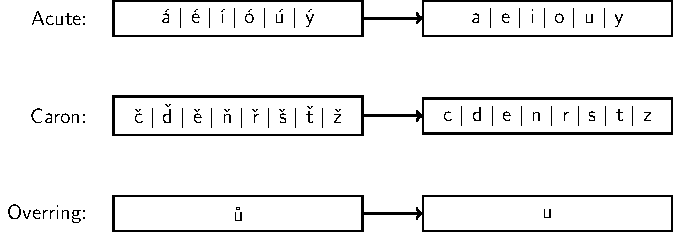
\includegraphics[scale=0.75]{src/fig/pdfs/tikz/diacritics_diacriticless.pdf}
        \caption{Creation of diacriticless corpus.}
      \end{figure}     
    \end{column}
  \end{columns}
\end{frame}


% Balanced models
\begin{frame}
  \frametitle{Results: Balanced models}
  \textcolor{cvut_navy}{\textbf{Results analysis}}
  \begin{itemize}
    \item Supervised learning enhance model performance.
    \item English models work well for Czech too.    
    \item Task-specified fine-tuning boosts performance. 
  \end{itemize}
  \begin{table}
    \centering
    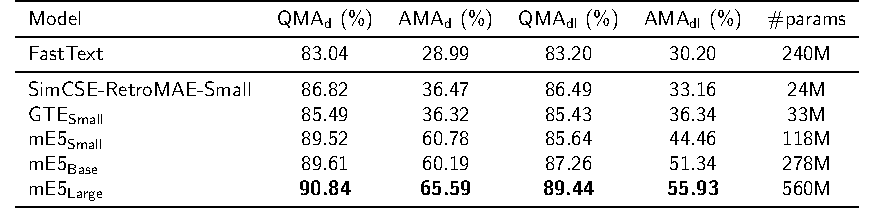
\includegraphics[scale=0.8]{src/fig/pdfs/tables/balanced.pdf}
    \caption{Balanced models compared to baseline.}
  \end{table}
\end{frame}


% Retrieval-Augmented Generation (RAG)
\begin{frame}
  \frametitle{Retrieval-Augmented Generation (RAG)}
  \begin{columns}[onlytextwidth,T]
    \begin{column}{0.75\textwidth}
      \begin{figure}[h]
        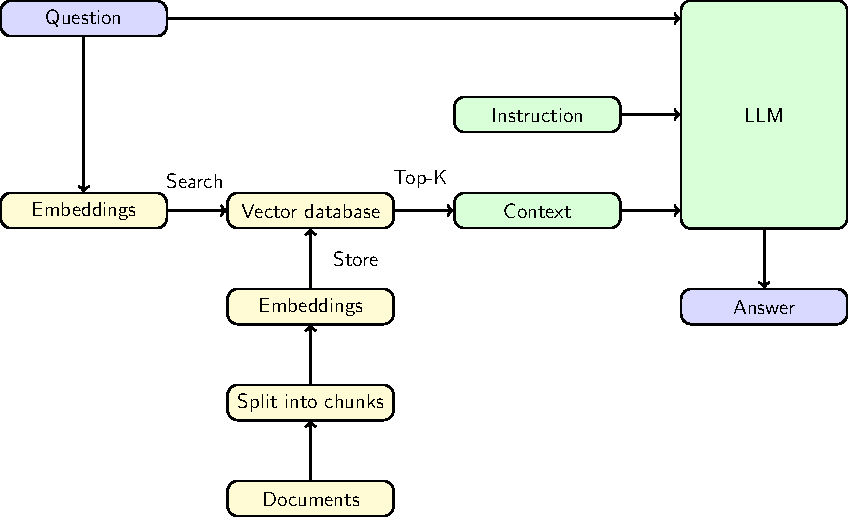
\includegraphics[scale=0.6]{src/fig/pdfs/tikz/RAG_scheme.pdf}
        \caption{RAG architecture.}
       \end{figure}
    \end{column}

    \begin{column}{0.75\textwidth}
      \vspace{10px}
      \textcolor{cvut_navy}{\textbf{Factors}}
      \begin{itemize}
        \item Embedding \\model
        \item Chunk size
      \end{itemize}
    \end{column}
  \end{columns}
\end{frame}


% Optimizing RAG
\begin{frame}
  \frametitle{Results: RAG optimization}
  \textcolor{cvut_navy}{\textbf{RAG Components}}
  \begin{itemize}
    \item Embedding model: GTE\textsubscript{Small}.
    \item Chunks: 256, 512, 1024, 2048, 4096 symbols.
    \item Almost same context size (3072 - 4096 symbols).
    \item Answers generation: GPT-3.5-turbo.
    \item Answers quality measurement: GPT-4o.
  \end{itemize}
  
  \begin{table}
    \begin{table}[ht!]
    \centering
    \begin{tabular}{lc|ccc}
      \toprule
      $S_{chunk}$ & $K$ & ACC (\%) & $t_{mean}$ \\
      \midrule
      256  & 12 & 43.5 & 132s \\
      512  & 6  & 57.5 & 162s \\
      1024 & 3  & 64.5 & 162s \\
      2048 & 2  & 64.0 & 111s \\
      4096 & 1  & \textbf{67.0} & \textbf{83s} \\
      \bottomrule
    \end{tabular}
    \label{tab:RAG_evaluation}
\end{table}
    
    \caption{RAG evaluation.}
  \end{table}
\end{frame}


% Summary
\placelogofalse 
\begin{frame}
  \frametitle{Summary}
  \textcolor{cvut_navy}{\textbf{Summary}}
  \begin{itemize}
    \item Transformer models has better performance, that tractional embedding models.
    \item Best embedding models: SimCSE-RetroMAE-Small, GTE\textsubscript{Small}, all mE5 verions.
    \item Best embedding model overall: mE5\textsubscript{Large}.
    \item Best chunk size for RAG: 4096 symbols.
  \end{itemize}
  \vspace{10px}
  \begin{center}
    \huge \textcolor{cvut_navy}{\textbf{Thank you for your attention!}}  
  \end{center}
  \vspace{10px}
  \begin{center}
    
\includegraphics[height=2cm]{src/fig/pdfs/ctu_logo_blue_filled.pdf}
  \end{center}
\end{frame}

% Questions
\placelogotrue
\begin{frame}
  \frametitle{Questions}
  \textcolor{cvut_navy}{\textbf{Opponent}}: Ing. Luboš Král, Ph.D.

  \vspace{20px}

  \textcolor{cvut_navy}{\textbf{Question 1.}} What is the main use of RAG systems?
  \begin{itemize}
    \item Improved accuracy and up-to-date information from external sources for question answering.
    \item Content creation and summarization.
    \item Documents analysis.
  \end{itemize}
  \textcolor{cvut_navy}{\textbf{Question 2.}} By how much does the accuracy of RAG systems for Czech fall short of English?
  % \begin{itemize}
    % \item There is not the exact answer for Czech language
    % \item ~8\%-12\% difference between RAG systems in English and Polish (relative to Czech gramatics and language structure).
    % \item Polish has 5x more native speakers, so 
  % \end{itemize}
\end{frame}

\end{document}
% =============================================================
% =========================== END =============================
% =============================================================

